\documentclass{article}
\usepackage{amsmath}
\usepackage{physics}
\usepackage{graphicx}
\title{PSET 1}
\author{Patryk Kozlowski}
\date{\today}

\begin{document}
\maketitle
\section{Problem 1: Adjoint Operators and Turnover Rule (10 points)}
\subsubsection{Question}
Two operators $\hat{O}$ and $\hat{O}^\dagger$ are defined to be adjoint if their expectation values are complex conjugates of one another. That is:
\begin{equation*}
    \expval{\hat{O}^\dagger}{\phi} = \expval{\hat{O}}{\phi}^*
\end{equation*}
and
\begin{equation*}
    (\hat{O}^\dagger)^\dagger = \hat{O}
\end{equation*}

Consider two functions $\phi_1$ and $\phi_2$ in the domain of adjoint operators $\hat{O}$ and $\hat{O}^\dagger$. Two new functions in this domain, $\Phi_A$ and $\Phi_B$, are given by
\begin{align*}
    \Phi_A &= \phi_1 + \phi_2 \\
    \Phi_B &= \phi_1 + i\phi_2
\end{align*}
where $i = \sqrt{-1}$. Use the definition of adjoint operators to prove the turnover rule:
\begin{equation*}
    \bra{\phi _{1}}\hat{O}^\dagger\ket{\phi _{2}}= \bra{\hat{O} \phi _{1}}\ket{\phi _{2}}
\end{equation*}
Some important properties: if $z_1$ and $z_2$ are two different complex numbers, then $z_1^*z_2=(z_2z_1^*)^*$; $z^\dagger = z^*$; $\bra{u}^\dagger = \ket{u}$; $\bra{u_1}\ket{u_2}^\dagger= \bra{u_1}\ket{u_2}^*= \bra{u_2}\ket{u_1}$.

\subsubsection{Answer}
We consider
\begin{equation}
    \bra{\Phi _{A}}\hat{O}^\dagger\ket{\Phi _{A}}= \bra{\Phi _{A}} \hat{O}\ket{\Phi _{A}}^*
\end{equation}
and
\begin{equation}
    \bra{\Phi _{B}}\hat{O}^\dagger\ket{\Phi _{B}}= \bra{\Phi _{B}} \hat{O}\ket{\Phi _{B}}^*
\end{equation}
We insert that expressions for $\Phi_A$ and $\Phi_B$. For the first one, we have:
\begin{equation}
    \bra{\phi _{1} + \phi _{2}}\hat{O}^\dagger\ket{\phi _{1} + \phi _{2}}= \bra{\phi _{1} + \phi _{2}} \hat{O}\ket{\phi _{1} + \phi _{2}}^*
\end{equation}
Expanding both sides:
\begin{equation}
    \bra{\phi _{1}}\hat{O}^\dagger\ket{\phi _{1}} + \bra{\phi _{2}}\hat{O}^\dagger\ket{\phi _{2}} + \bra{\phi _{1}}\hat{O}^\dagger\ket{\phi _{2}} + \bra{\phi _{2}}\hat{O}^\dagger\ket{\phi _{1}} = \left(\bra{\phi _{1}} \hat{O}\ket{\phi _{1}} + \bra{\phi _{2}} \hat{O}\ket{\phi _{2}} + \bra{\phi _{1}} \hat{O}\ket{\phi _{2}} + \bra{\phi _{2}} \hat{O}\ket{\phi _{1}}\right)^*
\end{equation}
Distributing out the complex conjugation:
\begin{equation}
    \bra{\phi _{1}}\hat{O}^\dagger\ket{\phi _{1}} + \bra{\phi _{2}}\hat{O}^\dagger\ket{\phi _{2}} + \bra{\phi _{2}}\hat{O}^\dagger\ket{\phi _{1}} + \bra{\phi _{1}}\hat{O}^\dagger\ket{\phi _{2}} = \bra{\phi _{1}} \hat{O}\ket{\phi _{1}}^* + \bra{\phi _{2}} \hat{O}\ket{\phi _{2}}^* + \bra{\phi _{2}} \hat{O}\ket{\phi _{1}}^* + \bra{\phi _{1}} \hat{O}\ket{\phi _{2}}^*
\end{equation}
We can cancel out the first two terms from either side:
\begin{equation}
    \bra{\phi _{2}}\hat{O}^\dagger\ket{\phi _{1}} + \bra{\phi _{1}}\hat{O}^\dagger\ket{\phi _{2}} = \bra{\phi _{2}} \hat{O}\ket{\phi _{1}}^* + \bra{\phi _{1}} \hat{O}\ket{\phi _{2}}^*
\end{equation}
For the second one, we have:
\begin{equation}
    \bra{\phi _{1} + i\phi _{2}}\hat{O}^\dagger\ket{\phi _{1} + i\phi _{2}}= \bra{\phi _{1} + i\phi _{2}} \hat{O}\ket{\phi _{1} + i\phi _{2}}^*
\end{equation}
Expanding both sides:
\begin{align*}
    \bra{\phi _{1}}\hat{O}^\dagger\ket{\phi _{1}} + \bra{\phi _{2}}\hat{O}^\dagger\ket{\phi _{2}} + i\bra{\phi _{1}}\hat{O}^\dagger\ket{\phi _{2}} -i \bra{\phi _{2}}\hat{O}^\dagger\ket{\phi _{1}} &= \\ \left(\bra{\phi _{1}} \hat{O}\ket{\phi _{1}} + \bra{\phi _{2}} \hat{O}\ket{\phi _{2}} + i\bra{\phi _{1}} \hat{O}\ket{\phi _{2}} -i \bra{\phi _{2}} \hat{O}\ket{\phi _{1}}\right)^*
\end{align*}
Distributing out the complex conjugation:
\begin{equation}
    \bra{\phi _{1}}\hat{O}^\dagger\ket{\phi _{1}} + \bra{\phi _{2}}\hat{O}^\dagger\ket{\phi _{2}} + i\bra{\phi _{1}}\hat{O}^\dagger\ket{\phi _{2}} -i \bra{\phi _{2}}\hat{O}^\dagger\ket{\phi _{1}} = \bra{\phi _{1}} \hat{O}\ket{\phi _{1}}^* + \bra{\phi _{2}} \hat{O}\ket{\phi _{2}}^* - i\bra{\phi _{1}} \hat{O}\ket{\phi _{2}}^* +i \bra{\phi _{2}} \hat{O}\ket{\phi _{1}}^*
\end{equation}
We can cancel out the first two terms from both sides:
\begin{equation}
    i\bra{\phi _{1}}\hat{O}^\dagger\ket{\phi _{2}} -i \bra{\phi _{2}}\hat{O}^\dagger\ket{\phi _{1}} = - i\bra{\phi _{1}} \hat{O}\ket{\phi _{2}}^* +i \bra{\phi _{2}} \hat{O}\ket{\phi _{1}}^*
\end{equation}
Multiplane through equation 6 by $i$ and adding it to 9, then dividing the result by $2i$, we get:
\begin{equation}
    \bra{\phi _{1}}\hat{O}^\dagger\ket{\phi _{2}} = \bra{\phi _{2}} \hat{O}\ket{\phi _{1}}^*
\end{equation}
So, we have shown the turnover rule that:
\begin{equation}
    \bra{\phi _{1}}\hat{O}^\dagger\ket{\phi _{2}}= \bra{\hat{O} \phi _{1}}\ket{\phi _{2}}
\end{equation}


\section{Problem 2: Dynamical Quantity $F$ and Time-Dependent Schrödinger Equation (10 points)}
\subsubsection{Question}
Consider a dynamical quantity $F$ given by the expectation value of the operator $\hat{F}$:
\begin{equation*}
    \langle F \rangle = \int_{-\infty}^{\infty} \Psi^*(x, y, z, t)\hat{F}\Psi(x, y, z, t)\,d\tau 
\end{equation*}
Use the time-dependent Schrödinger equation and the turnover rule to prove that:
\begin{equation*}
    \frac{d\langle F \rangle}{dt} = \frac{i}{\hbar} \int_{-\infty}^{\infty} \Psi^*(x, y, z, t)(\hat{H}\hat{F} - \hat{F}\hat{H})\Psi(x, y, z, t)\,d\tau
\end{equation*}
where $\hat{H}$ is the Hamiltonian operator and $\hbar$ is Planck's constant divided by $2\pi$.

\subsubsection{Answer}
We start by considering:
\begin{equation}
    \frac{d\langle F \rangle}{dt} = \frac{d}{dt}\int_{-\infty}^{\infty} \Psi^*(x, y, z, t)\hat{F}\Psi(x, y, z, t)\,d\tau = \int_{-\infty}^{\infty} \frac{\partial}{\partial t}\left(\Psi^*(x, y, z, t)\hat{F}\Psi(x, y, z, t)\right)\,d\tau
\end{equation}
We can distribute the deferential:
\begin{equation}
    = \int_{-\infty}^{\infty} \left(\frac{\partial \Psi^*(x, y, z, t)}{\partial t}\hat{F}\Psi(x, y, z, t) + \Psi^*(x, y, z, t)\frac{\partial \hat{F}}{\partial t}\Psi(x, y, z, t) + \Psi^*(x, y, z, t)\hat{F}\frac{\partial \Psi(x, y, z, t)}{\partial t}\right)\,d\tau
\end{equation}
Now, the time dependent Schrödinger equation tells us that:
\begin{equation}
    i\hbar \frac{\partial \Psi(x, y, z, t)}{\partial t} = \hat{H}\Psi(x, y, z, t)
\end{equation}
and taking the complex conjugate of both sides gives us:
\begin{equation}
    -i\hbar \frac{\partial \Psi^*(x, y, z, t)}{\partial t} = \Psi^*(x, y, z, t)\hat{H}
\end{equation}
We can substitute this in and use the fact that F should be time independent:
\begin{equation}
    = \int_{-\infty}^{\infty} \frac{i}{\hbar} \left(\Psi^*(x, y, z, t)\hat{H}\hat{F}\Psi(x, y, z, t) - \Psi^*(x, y, z, t)\hat{F}\hat{H}\Psi(x, y, z, t)\right)\,d\tau
\end{equation}
So, we have arrived at the desired versal of:
\begin{equation}
    = \frac{i}{\hbar} \int_{-\infty}^{\infty} \Psi^*(x, y, z, t)(\hat{H}\hat{F} - \hat{F}\hat{H})\Psi(x, y, z, t)\,d\tau
\end{equation}
\section{Problem 3: Orbital Angular Momentum Operators and Commutators (10 points)}
\subsubsection{Question}
Use the definitions of the orbital angular momentum operators $\hat{L}_x$, $\hat{L}_y$, and $\hat{L}_z$ to derive the following commutators:
\begin{align*}
    [\hat{L}_x, \hat{L}_y] &= i\hbar\hat{L}_z \\
    [\hat{L}_y, \hat{L}_z] &= i\hbar\hat{L}_x \\
    [\hat{L}_z, \hat{L}_x] &= i\hbar\hat{L}_y
\end{align*}

\subsubsection{Answer}
We know that we have:
\begin{align*}
    \hat{L}_x &= \hat{y}\hat{p}_z - \hat{z}\hat{p}_y \\
    \hat{L}_y &= \hat{z}\hat{p}_x - \hat{x}\hat{p}_z \\
    \hat{L}_z &= \hat{x}\hat{p}_y - \hat{y}\hat{p}_x
\end{align*}
So, evaluating the commutator $[\hat{L}_x, \hat{L}_y]$:
\begin{equation}
    \begin{split}
        [\hat{L}_x, \hat{L}_y] &= [\hat{y}\hat{p}_z - \hat{z}\hat{p}_y, \hat{z}\hat{p}_x - \hat{x}\hat{p}_z] \\
        &= [\hat{y}\hat{p}_z, \hat{z}\hat{p}_x] - [\hat{y}\hat{p}_z, \hat{x}\hat{p}_z] - [\hat{z}\hat{p}_y, \hat{z}\hat{p}_x] + [\hat{z}\hat{p}_y, \hat{x}\hat{p}_z]
    \end{split}
\end{equation}
Sense the only terms that fail to commute are $x$ with $p_x$, $y$ with $p_y$, and $z$ with $p_z$, the middle to terms drop out, leaving:
\begin{equation}
    = [\hat{y}\hat{p}_z, \hat{z}\hat{p}_x] + [\hat{z}\hat{p}_y, \hat{x}\hat{p}_z]\\
= \hat{y}\hat{p}_x[\hat{p}_z, \hat{z}] + \hat{x}\hat{p}_y[\hat{z}, \hat{p}_z]\\
\end{equation}
Now we can use the canonical commutation relation $[\hat{z}, \hat{p}_z] = i\hbar$ to get:
\begin{equation}
    = \hat{y}\hat{p}_x(-i\hbar) + \hat{x}\hat{p}_y(i\hbar)\\
= i\hbar(\hat{x}\hat{p}_y - \hat{y}\hat{p}_x)\\
= i\hbar\hat{L}_z
\end{equation}
Cyclic permutation of the indices gets as the other commutators.




\section{Problem 4: Linear Momentum Operator and Hermitian Property (10 points)}
\subsubsection{Question}
The linear momentum operator is $\hat{p}_x = -i\hbar \frac{\partial}{\partial x}$. Use integration by parts in the following integral to prove that $\hat{p}_x$ is Hermitian (i.e., self-adjoint).
\begin{equation*}
    \int_{-\infty}^{+\infty} \left(-i\hbar \frac{\partial \phi_1}{\partial x}\right)^* \phi_2 \, dx
\end{equation*}
where the wavefunctions $\phi_1$ and $\phi_2$ vanish at $\pm\infty$.

\subsubsection{Answer}
To start with, we will move the constant terms out in front of the integral:
\begin{equation}
    \begin{split}
        \int_{-\infty}^{+\infty} \left(-i\hbar \frac{\partial \phi_1}{\partial x}\right)^* \phi_2 \, dx &= (-i\hbar)^* \int_{-\infty}^{+\infty} \left(\frac{\partial \phi_1}{\partial x}\right)^* \phi_2 \, dx \\
        &= i\hbar \int_{-\infty}^{+\infty} \left(\frac{\partial \phi_1}{\partial x}\right)^* \phi_2 \, dx
    \end{split}
\end{equation}
Choosing $u=\phi_2$ and $dv=\left(\frac{\partial \phi_1}{\partial x}\right)^*$, we have $du=\frac{\partial \phi _{2}}{\partial x}$ and $v=\phi_1^*$. So, we have:
\begin{equation}
    \begin{split}
        \int_{-\infty}^{+\infty} \left(-i\hbar \frac{\partial \phi_1}{\partial x}\right)^* \phi_2 \, dx &= i\hbar \left(\phi_1^*\phi_2\right)_{-\infty}^{+\infty} - i\hbar \int_{-\infty}^{+\infty} \phi_1^* \frac{\partial \phi_2}{\partial x} \, dx \\
        &= 0+\int_{-\infty}^{+\infty} \phi_1^* \left(-i\hbar \frac{\partial \phi_2}{\partial x}\right) \, dx \\
    \end{split}
\end{equation}
So, indeed we have shown that 
\begin{equation}
    \bra{\phi _{1}}\hat{p}_x\ket{\phi _{2}} = \bra{\phi _{2}}\hat{p}_x\ket{\phi _{1}}^*
\end{equation}
with equation 5 on the left and the integral in the question on the right.
$\hat{p}_x$ being the transpose contract of itself is the definition of Hermiticity.
\section{problem 5}
\subsection{Answer}
\begin{equation}
    \frac{dN_{k}}{dt} = A N_l + B N_l \rho (v_{kl})-BN_k \rho (v_{kl})
\end{equation}
for the oder state, we would have:
\begin{equation}
    \frac{dN_{l}}{dt} = -A N_l - B N_l \rho (v_{kl})+BN_k \rho (v_{kl})
\end{equation}
\subsection{Answer}
We want to change equation 24 to a single variable, by substituting $N_k = N_{Total} - N_l$ into the first equation, we get:
\begin{equation}
    \frac{dN_{l}}{dt} = -A N_l - B N_l \rho (v_{kl})+B(N_{Total} - N_l) \rho (v_{kl})
\end{equation}
 Grouping together the factors of $N_l$ and $N_{Total}$, we get:
    \begin{equation}
        \frac{dN_{l}}{dt} = -A N_l + B N_{Total} \rho (v_{kl}) - 2BN_l \rho (v_{kl}) = B N_{Total} \rho (v_{kl}) - (A+2B\rho (v_{kl}))N_l
    \end{equation}
This reminds us of $\frac{dx}{dt} + \alpha(t)  x = \beta(t) $, so we can use the integrating factor method with $\alpha(t) = A+2B\rho (v_{kl})$ and $\beta(t) = B N_{Total} \rho (v_{kl})$ with the integrating factor $\mu (t) = e^{\int \alpha dt} = e^{(A+2B\rho (v_{kl}))t}$ to get:
\begin{equation}
    \frac{d}{dt}(N_l e^{(A+2B\rho (v_{kl}))t}) = B N_{Total} \rho (v_{kl})e^{(A+2B\rho (v_{kl}))t}
\end{equation}
Now, we can integrate on both sides with respect to t:
\begin{equation}
    N_l e^{(A+2B\rho (v_{kl}))t} = \int B N_{Total} \rho (v_{kl})e^{(A+2B\rho (v_{kl}))t} dt = \frac{B N_{Total} \rho (v_{kl})}{A+2B\rho (v_{kl})}e^{(A+2B\rho (v_{kl}))t} + C
\end{equation}
Solving for $N_l$:
\begin{equation}
    N_l = \frac{B N_{Total} \rho (v_{kl})}{A+2B\rho (v_{kl})} + Ce^{-(A+2B\rho (v_{kl}))t}
\end{equation}
Now, we can use the initial condition $N_l(0) = 0$ to solve for C:
\begin{equation}
    0 = \frac{B N_{Total} \rho (v_{kl})}{A+2B\rho (v_{kl})} + C
\end{equation}
Rearranging, we get:
\begin{equation}
    C = -\frac{B N_{Total} \rho (v_{kl})}{A+2B\rho (v_{kl})}
\end{equation}
So, we have:
\begin{equation}
    N_l(t) = \frac{B N_{Total} \rho (v_{kl})}{A+2B\rho (v_{kl})}\left(1-e^{-(A+2B\rho (v_{kl}))t}\right)
\end{equation}
Since $N_k = N_{Total} - N_l$, we have:
\begin{equation}
    N_k(t) = N_{Total} - \frac{B N_{Total} \rho (v_{kl})}{A+2B\rho (v_{kl})}\left(1-e^{-(A+2B\rho (v_{kl}))t}\right)
\end{equation}
\subsection{Answer}
As $t \rightarrow \infty$, we have:
\begin{equation}
    N_l(t) \rightarrow \frac{B N_{Total} \rho (v_{kl})}{A+2B\rho (v_{kl})}
\end{equation}
and
\begin{equation}
    N_k(t) \rightarrow N_{Total} - \frac{B N_{Total} \rho (v_{kl})}{A+2B\rho (v_{kl})} = N_{Total}\left(1-\frac{B \rho (v_{kl})}{A+2B\rho (v_{kl})}\right)
\end{equation}
\subsection{Answer}
Consider the limit as $t \rightarrow \infty$ of $\frac{N_l(t)}{N_{Total}}$:
\begin{equation}
    \frac{N_l(t)}{N_{Total}} \rightarrow \frac{B \rho (v_{kl})}{A+2B\rho (v_{kl})}
\end{equation}
No matter how you increase $\rho (v_{kl})$, the fraction will never be greater than $\frac{B}{2B} = \frac{1}{2}$. So, the fraction of atoms in the excited state will never be greater than $\frac{1}{2}$. So the answer is no.
\section{Problem 6: Spectral Analysis of Sunlight}

\subsubsection{Question (a)}
Make an overlay plot of intensity vs. wavelength of the two spectra using the units provided in the file.

\subsubsection{Answer (a)}
To plot the overlay of the two spectra, I used some Python code with pandas and matplotlib:
% I want to include a png plot that is in the same directory as this file
\begin{figure}[h]
    \centering
    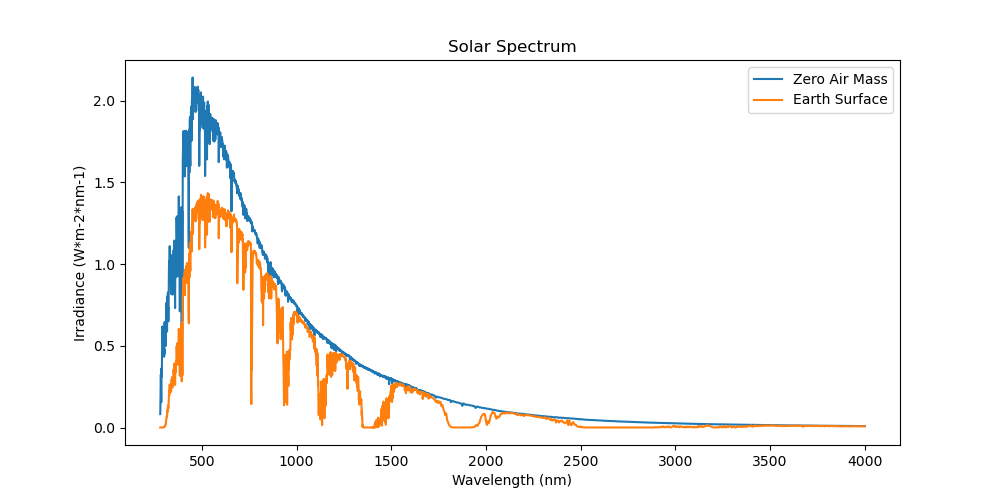
\includegraphics[width=\textwidth]{solar_spectrum.png}
\end{figure}



\subsubsection{Question (b)}
What fraction of the light power at the Earth's surface is in the visible spectral region (400-700 nm)?

\subsubsection{Answer (b)}
Using my python script, I found this to be: 0.4233848887511344


\subsubsection{Question (c)}
Use Planck's equation for the energy of a photon (\(E = hv\)) to make a new overlay plot of photon flux vs. wavelength of the two spectra using flux units of Einsteins per second per square meter per nanometer (Einsteins\(^{-1}\)m\(^{-2}\)nm\(^{-1}\)). The Einstein unit is defined to be 1 mole of photons.

\subsubsection{Answer (c)}
We need to formulate an equation that will let us convert from Watts per square meter per nanometer to Einsteins\(^{-1}\)m\(^{-2}\)nm\(^{-1}\). We know that:
\begin{equation}
    E = hv = \frac{hc}{\lambda}
\end{equation}
So, we can use this to get the energy of a photon at a given wavelength.
\begin{figure}[h]
    \centering
    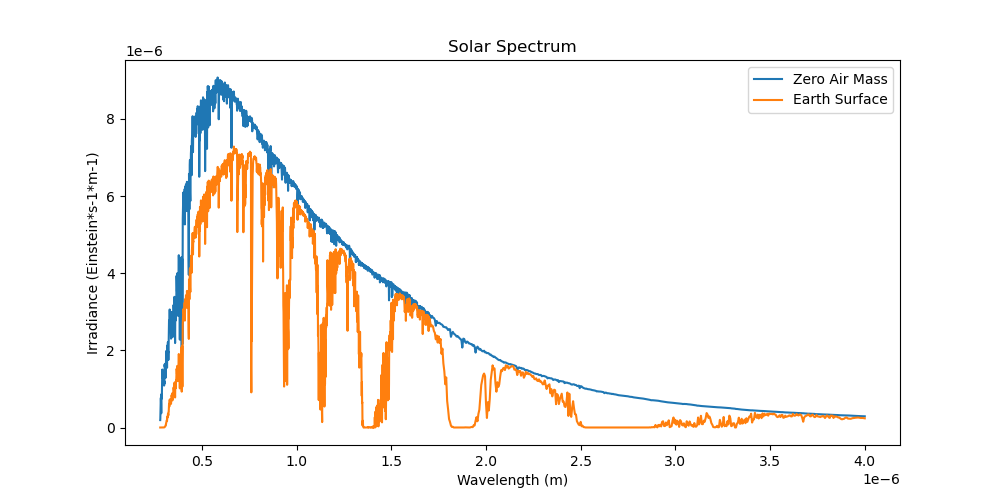
\includegraphics[width=\textwidth]{einstein.png}
\end{figure}



\subsubsection{Question (d)}
What fraction of the photons reaching the Earth's surface is in the visible spectral region (400-700 nm)?

\subsubsection{Answer (d)}
To find the fraction of photons in the visible region, we perform the calculation using a similar python script: 0.29372284127095055
% Include Python code snippet or mathematical derivation here.

\subsubsection{Question (e)}
The light absorbance of a sample is defined by the equation: Abs = \(-\log_{10}(\frac{I}{I_0})\), where \(I_0\) is the intensity of light incident on the sample and \(I\) is the intensity of transmitted through the sample. Use the data in the Excel file to plot the absorbance as a function of wavelength for the atmosphere.

\subsubsection{Answer (e)}
The absorbance of the atmosphere is plotted as a function of wavelength:
\begin{figure}[h]
    \centering
    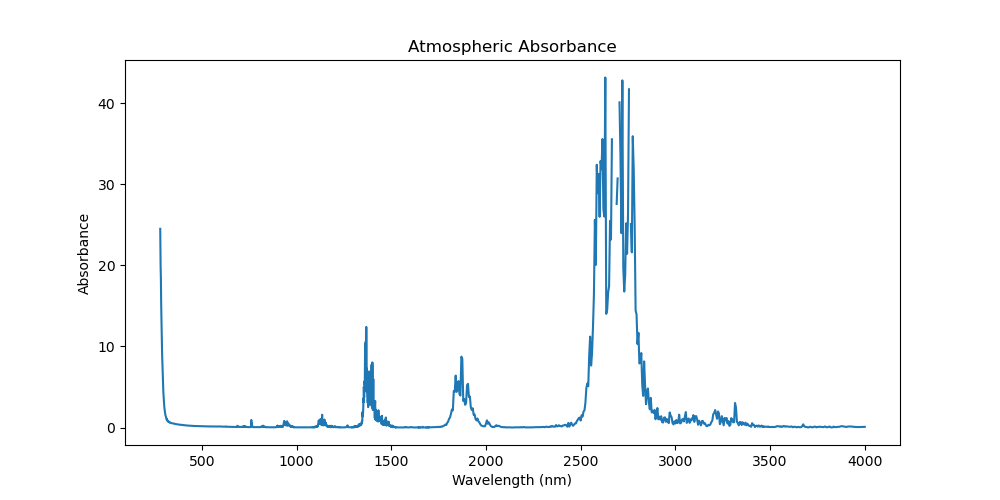
\includegraphics[width=\textwidth]{absorbance_corrected.png}
\end{figure}

\end{document}
